%\documentclass[a4paper,12pt]{eskdtext}		%размер бумаги устанавливаем А4, шрифт 12пунктов
\documentclass[a4paper,14pt]{scrartcl}		%размер бумаги устанавливаем А4, шрифт 12пунктов
%\documentclass[14pt,a4paper,twoside]{report}
\usepackage[T2A]{fontenc}
\usepackage[utf8]{inputenc}			%включаем свою кодировку: koi8-r или utf8 в UNIX, cp1251 в Windows
\usepackage[english,russian]{babel}		%используем русский и английский языки с переносами
\usepackage{amssymb,amsfonts,amsmath,mathtext,cite,enumerate,float} %подключаем нужные пакеты расширений
\usepackage[dvips]{graphicx}			%хотим вставлять в диплом рисунки?
\usepackage{soul}
\usepackage[14pt]{extsizes}

\graphicspath{{images/}}			%путь к рисункам

\makeatletter
\renewcommand{\@biblabel}[1]{#1.} 		% Заменяем библиографию с квадратных скобок на точку:
\makeatother

%\renewcommand\large{\@setfontsize\large{15.5}{17}}
%\renewcommand\Large{\@setfontsize\Large{16.5}{19}}
%\renewcommand\small{\@setfontsize\small{9}{9.5}}

\usepackage{geometry} 				% Меняем поля страницы
\geometry{left=2cm}				% левое поле
\geometry{right=1.4cm}				% правое поле
\geometry{top=1cm}				% верхнее поле
\geometry{bottom=2cm}				% нижнее поле

\renewcommand{\theenumi}{\arabic{enumi}}	% Меняем везде перечисления на цифра.цифра
\renewcommand{\labelenumi}{\arabic{enumi}}	% Меняем везде перечисления на цифра.цифра
\renewcommand{\theenumii}{\arabic{enumii}}	% Меняем везде перечисления на цифра.цифра
\renewcommand{\labelenumii}{\arabic{enumi}.\arabic{enumii}.}% Меняем везде перечисления на цифра.цифра
\renewcommand{\theenumiii}{\arabic{enumiii}}	% Меняем везде перечисления на цифра.цифра
\renewcommand{\labelenumiii}{\arabic{enumi}.\arabic{enumii}.\arabic{enumiii}.}% Меняем везде перечисления на цифра.цифра

\begin{document}
%\begin{titlepage}
\newpage

% title page with the name of the university

\begin{center}
\textbf{Федеральное агентство по образованию} \\
\vspace{0.5cm}
\fontsize{10pt}{10.5pt}{\fontseries{b}\selectfont{Государственное образовательное учреждение высшего профессионального образования} }\\
\fontsize{12pt}{12.5pt}{\fontseries{b}\selectfont{“Московский государственный университет приборостроения и информатики”} }\\*
%\hrulefill
\end{center}

\begin{center}
Факультет ИТ  Направление 230105 \\
Кафедра ИТ-6 «Управление и моделирование систем» Квалификация инженер \\
\end{center}

\begin{flushright}
\textit{Утверждаю} \\
Зав. кафедрой \\
\rule{2.9cm}{0.5pt} Мацнев А.П. \\
«\rule{1cm}{0.5pt}»\rule{3cm}{0.5pt} 2010г.
\end{flushright}

\vfill
			% add header

\begin{center}
\textbf{\Large ПОЯСНИТЕЛЬНАЯ ЗАПИСКА \\
к дипломному проекту на тему: }
\end{center}

\vfill\vfill

\begin{center}
\textsc{\textbf{ничо не секу\linebreak ваще}}
\end{center}

\vfill\vfill

\begin{flushleft}
Дипломник \hrulefill Никифоров А.А \\
Группа \hrulefill   шифр \hrulefill \\
Обозначение проекта (работы) \hrulefill \\
\vfill
\textbf{Руководитель проекта (работы) \hrulefill}
\vfill
\begin{center}
Консультанты по разделам:
\end{center}
Наименование разделов: \\
\hrulefill \\
\hrulefill \\
\hrulefill \\
Нормоконтроль \hrulefill \\
\end{flushleft}

\vspace{\fill}

\begin{center}
Москва 2010г.
\end{center}

\end{titlepage}
					% это титульный лист
%\begin{titlepage}
\newpage

% title page with the name of the university

\begin{center}
\textbf{Федеральное агентство по образованию} \\
\vspace{0.5cm}
\fontsize{10pt}{10.5pt}{\fontseries{b}\selectfont{Государственное образовательное учреждение высшего профессионального образования} }\\
\fontsize{12pt}{12.5pt}{\fontseries{b}\selectfont{“Московский государственный университет приборостроения и информатики”} }\\*
%\hrulefill
\end{center}

\begin{center}
Факультет ИТ  Направление 230105 \\
Кафедра ИТ-6 «Управление и моделирование систем» Квалификация инженер \\
\end{center}

\begin{flushright}
\textit{Утверждаю} \\
Зав. кафедрой \\
\rule{2.9cm}{0.5pt} Мацнев А.П. \\
«\rule{1cm}{0.5pt}»\rule{3cm}{0.5pt} 2010г.
\end{flushright}

\vfill
		% add header

\end{titlepage}

\tableofcontents 				% это оглавление, которое генерируется автоматически
\newpage
%\section{ИССЛЕДОВАТЕЛЬСКИЙ РАЗДЕЛ}

% =========================== 1.1
\subsection{Постановка задачи}
Главной задачей данной дипломной работы ставится разработка программно-аппаратной платформы для захвата сигнала системы спутниковой 
навигации Navstar GPS. Результатом дипломной работы станет разработанное ПО для FGPA микросхемы, реализующее интерфейс взаймодействия с ПК,
интерфейс программирования GPS-микросхемы, интерфейс управления микросхемой памяти, а также набор тестов для валидации корректной работы
платы. Вместе с этим, будет разработано ПО управления платой с ПК, ПО предоставления сигнала в публично доступные источники
(ftp, nfs, samba), а также ПО захвата и сопровождения сигналов спутниковой навигации. 

Дополнительной целью является максимально возможная ориентация проекта на академическую среду. Что подразумевает открытие кода и прошивок
для пользователей, разработка простых и бесплатных средств обработки сигнала. Результаты работы платы должны иметь возможность
автоматической публикации на публичные носители как по расписанию, так и по команде оператора. Дампы сигналов должны снабжаться
комментариями для возможности корректной обработки как на программных платформах (ПК), так и на аппаратных (ПЛИС).

\subsection{Параметры сигнала GPS}
\label{razdel11}
\subsubsection*{Частота передачи}
Сигнал GPS состоит из двух частотных компонент: link 1 (L1) и link 2 (L2). Центром частотного спектра L1 является
частота 1575.42 МГц и центром частотного спектра L2 является частота 1227.6 Мгц. Эти частоты когерентны с
частотой 10.23 МГц. Они могут быть получены как:

\begin{equation}
L1=1575.42\mbox{МГц}=154*10.23\mbox{МГц}
\label{eq:l1_freq}
\end{equation}

\begin{equation}
L2=1227.6\mbox{МГц}=120*10.23\mbox{Мгц}
\label{eq:l2_freq}
\end{equation}

Частоты генерируются с высокой точностью. Сгенерированная частота немного ниже чем 10.23 МГц, для учета 
релятивисткского эффекта. Сдвиг частоты составляет ${-4.567\cdot10^{-3}\mbox{Гц}}$. Он согласован c долей
${-4.4647\cdot10^{-10}}$:

\begin{equation}
-4.567\cdot10^{-3}/10.23\cdot10^{6} = -4.4647\cdot10^{-10}
\end{equation}

По этой причине, используемая частота составляет 10.229999995433 МГц ${(10.23\cdot10^{6} - 4.567\cdot10^{-3})}$,
а не 10.23 МГц. Когда приемник принимает сигнал, он находится
на нужной частоте. Однако, движение спутника и приемника может создавать Допплеровский эффект. Частота Допплеровского
сдвига, создаваемого движением спутника, на частоте L1 составляет примерно ${\pm5\mbox{кГц}}$ \cite{yacenkov, tsui}.

Структура сигнала может поменяться в будущем, но на данный момент L1 частота содержит C/A и P(Y) сигналы, в то
время как L2 содержит только P(Y) сигнал. C/A и P(Y) сигналы на частоте L1 сдвинуты на 90 градусов
относительно друг-друга и могут быть записаны как:

\begin{equation}
S_{L1}=A_p P(t) D(t) cos(2\pi f_1 t + \phi) + A_c C(t) D(t) sin(2\pi f_1 t + \phi),
\label{eq:s_l1}
\end{equation}

где ${S_{L1}}$ - сигнал на L1 частоте, ${A_p}$ - амплитуда P-кода, ${P(t)=\pm 1}$ представлет фазу P-кода,
${D(t) = \pm 1}$ представляет данные, ${f_1}$ - L1 частота, ${\phi}$ - начальная фаза, ${A_c}$ - амплитуда C/A кода,
${C(t)} = \pm 1$ представляет фазу C/A кода.

\subsubsection*{C/A код}
GPS сигнал является фазо-манипулированным сигналом с ${\phi = 0, \pi}$. Такой вид расширения спектра называется бифазным 
(BPSK). Скорость изменения фаз соответствует скорости чипа. Форма спектра может быть описана как sinc-функция,
с шириной спектра пропорциональной скорости чипа. 

C/A код - бифазно-манипулированный сигнал со скоростью чипа 1.023 Мгц. Однако, ширина спектра главного лепестка составляет
2.046 МГц. Каждый чип имеет длительность 977.5 нс (1/1023МГц). Полный период кода составляет 1023 чипа. Со скоростью
чипа 1.023 МГц, 1023 чипа равны 1мс, таким образом C/A код имеет длинну 1 мс. Этот код повторяется каждую миллисекунду.
Спектр C/A кода представлен на рисунке \ref{pic:ca_spectrum}. На рисунке \ref{pic:gps_data_format} изображена структура GPS сообщения. 

Учитывая вышесказанное, чтобы найти начало C/A кода требуется запись продолжительностью 1 мс. Если нет Допплеровского
эффекта в принятом сигнале, тогда 1 мс содержит все 1023 чипа. Разные C/A коды соответствуют разным спутникам.
C/A код относится к семейству Gold кодов.

\begin{figure}[H]
\begin{center}
\scalebox{0.9}{
\includegraphics[width=1\linewidth]{./pics/ca_spectrum.eps}
}
\end{center}
\caption{Пример спектра C/A кода}
\label{pic:ca_spectrum}
\end{figure}

\begin{figure}[H]
\begin{center}
\scalebox{0.5}{\includegraphics[width=1\linewidth]{./pics/gps_data_format.eps}}
\end{center}
\caption{Cтруктура сообщений навигационной системы GPS NAVSTAR}
\label{pic:gps_data_format}
\end{figure}

На первой строке рисунка \ref{pic:gps_data_format} изображен C/A код
длинной 1023 чипа, его длительность составляет 1 мс. На второй строке представлен 1 бит данных, частота поступления
битов составляет 50 Гц, таким образом длинна 1 бита равна 20 мс. В третьей строке изображено одно слово, длинна слова
600 мс. Один подфрейм формируется из 10 слов, его длинна 6 с. В пятой строке изображена страница данных, ее длительность
составляет 30 с и она содержит 5 подфреймов. Полный цикл данных состоит из 25 страниц, длительность цикла 12.5 мин.
25 страниц представлены 1 суперфреймом.

Параметры, необходимые для нахождения положения, содержатся в первых трех подфреймах. Если удается получить эти 3
подфрейма с 4 или более спутников, позиция навигатора может быть определена.  Теоритически, можно захватить примерно
18 секунд данных с 4 спутников и этого будет достаточно для определения позиции. Однако, подфреймы с каждого спутника
поступают в приемник не одновременно. В реальной ситуации не известно когда начнется первый подфрейм. Гарантированным
временем получения первых трех подфреймов является 30 секунд (1 страница) данных. Учитывая это, необходимо иметь
минимум 30 секунд данных для определения координат приемника.

\subsubsection*{Генерирование C/A кода}
GPS C/A сигналы принадлежат к семейству кодов содержащих псевдослучайный шум (PRN codes), также известным как Gold коды.
Сигналы генерируются посредством умножения двух 1023 битных PRN-последовательностей G1 и G2. И G1 и G2 сгенерированы
посредством 10-ти битного сдвигового регистра, управляемого кварцом с частотой 1.023 МГц. На рисунке
\ref{pic:g1_g2_generators} изображены генераторы G1 и G2.

Основная операция в этих генераторах одинаковая, поэтому обсуждается только генератор G2. MLS (maximum-lengh sequense)
генератор можно сделать из сдвигового регистра с нужной обратной связью. Если сдвиговый регистр состоит из 10 бит,
длинна генерированной последовательности равна 1023 ${2^{10}-1}$. Цепь обратной связи формируется с элементами сложения
по модулю.

\begin{figure}[H]
\begin{center}
\includegraphics[width=1\linewidth]{./pics/g1_g2_generators.eps}
\end{center}
\caption{G1 и G2 генераторы}
\label{pic:g1_g2_generators}
\end{figure}

Операция сложение по модулю 2 отражена в таблице \ref{tab:mod2}. Когда 2 входа одинаковы - выход равен 0, в обратном
случае 1. Позиции цепей определяются шаблоном последовательности. Обратная связь G1 состоит из битов 3 и 10, как 
показано на рисунке \ref{pic:g1_g2_generators} и отражена полиномом ${G1=1 + x^{3} + x^{10}}$. Обратная связь G2
образуется из битов 2, 3, 6, 8, 9, 10 и соответствующий ей полином G2:
${G2=1 + x^{2} + x^{3} + x^{6} + x^{8} + x^{9} + x^{10}}$ 

\begin{table}[H]
\begin{center}
\caption{Сложение по модулю 2}
\label{tab:mod2}
\begin{tabular}{|c|c|c|c|}
	\hline
		Вход 1 & Вход 2 & Результат \\
	\hline
		0 & 0 & 0 \\
	\hline
		0 & 1 & 1 \\
	\hline
		1 & 0 & 1 \\
	\hline
		1 & 1 & 0 \\
	\hline
\end{tabular}
\end{center}
\end{table}

Как видно, выходное значение регистров используется как выходное значение последовательности. Обозначим этот выход, как
MLS-выход. Однако, регистор G2 не использует MLS-выход. Выход генератора G2 получается умножением по модулю 2
двух разрядов регистра G2. Этот выход является задержанной версией MLS-выхода. Задержка определяется позицией выходных
битов в G2.

На рисунке \ref{pic:ca_generator} представлен генератор C/A кода. Начальное значение всех битов устанавливается в 1.
Спутник определяется по отводам G2 генератора. Всего существует 37 уникальных отводов. Для спутников используется 32
значения, но на орбите находится только 24 спутника \cite{tsui}. Остальные 5 значений зарезервированы для наземной
передачи.

\begin{figure}[H]
\begin{center}
\includegraphics[width=1\linewidth]{./pics/ca_generator.eps}
\end{center}
\caption{Генератор кода C/A}
\label{pic:ca_generator}
\end{figure}

\subsubsection*{Навигационные сообщения}
Каждый штатно функционирующий навигационный спутник передает навигационное сообщение, содержащее оперативную и неоперативную
навигационную информацию. Эта информация предназначена как для проведения текущих навигационных определений, так и для
планирования будущих сеансов приема \cite{yacenkov}.

Оперативная информация относится к тому спутнику, с борта которого эта информация передается, и содержит следующие данные
\cite{yacenkov, tsui}:
\begin{itemize}
\item координаты и параметры орбиты спутника в фиксированный момент времени (эфемериды);
\item сдвиг шкалы времени спутника относительно земной шкалы;
\item относительный сдвиг несущей частоты излучаемого сигнала от номинального значения;
\item код метки времени, необходимый для синхронизации аппаратуры потребителя.
\end{itemize}

Неоперативная информация относится к СНС в целом и содержит альманах системы:
\begin{itemize}
\item данные о функциональном состоянии всех спутников (альманах состояния);
\item сдвиг шкалы времени каждого спутника относительно системной шкалы (альманах фаз);
\item параметры орбит всех спутников системы (альманах орбит);
\item поправку к шкале времени относительно UTC.
\end{itemize}


% ========================== 1.2
\subsection{Обзор решений в области захвата сигналов в системах беспроводной передачи}
\label{razdel12}
\subsubsection*{Общие понятия}
Захват данных(data acquisition - DAQ) - это процесс регистрации данных реального мира и преобразования полученных данных в 
числовой вид, который может быть обработан на ПК. Захват данных и системы захвата данных(data acquistion systems - DAS) подразумевает
преобразование аналоговых волн в дискретные числовые значения для последующей обработки \cite{ni_acq}. В системы захвата данных входят:

\begin{itemize}
\item сенсоры(таймеры и тд), которые конвертируют физические параметры в электрические сигналы;
\item схемы конвертации сигналов с сенсоров в формы пригодные для конвертирования в цифровой формат;
\item АЦП, которые конвертируют информацию со схем конвертации в цифровой формат;
\item системы синхронизации и предварительной обработки сигнала.
\end{itemize}

На рисунке \ref{pic:acq} отражена наиболее общая схема системы захвата сигналов. Есть датчики, аппаратное обеспечение,
преобразующее сигналы с сенсоров в сигналы пригодные для подачи на АЦП и есть набор управляющего и анализирующего ПО
на ПК \cite{ni_acq}.

\begin{figure}[H]
\center{\includegraphics[width=1\linewidth]{./pics/acq_scheme.eps}}
\caption{Системы захвата данных}
\label{pic:acq}
\end{figure}

Одной из существенных проблем при разработке устройств для анализа сигналов и непосредственной работе по анализу сигналов
является проблема повторяемости данных \cite{ni_article}. Для примера, при отладке ГЛОНАСС навигатора необходимо 
воспроизвести некоторую ситуацию, однажды полученную при захвате сигнала. Очевидно, что сделать это крайне сложно, потому
что сигнал меняется со временем и воспроизвести ситуацию практически невозможно. Хорошим решением данной задачи является
работа с сохраненным сигналом. В данном случае проблема воспроизведения ситуации сводится к повторной подаче сохраненного
сигнала на вход тестируемого устройства. В данный момент существует два способа получения сигнала для последующего анализа:
генерирование сигнала с заданными характеристиками, запись реального сигнала \cite{ni_article}.

\subsubsection*{Портативный анализатор сигналов WiMAX (SeaMAX Mobile WiMAX Analyzer)}
Данный анализатор является IEEE 802.16e-2005 OFDMA PHY Base станцией анализа сигналов. Данная станция 
позволяет выбрать ширину полосы пропускания и частоту дискретизации.
SeaMAX Mobile предоставляет гибкую систему конфигурирования параметров PHY, таких как
размер БПФ и циклического префикса или выбрать опцию автоматического выбора данных параметров. Импорт IQ сигналов
из .txt файлов. Анализатор позволяет сохранять декодированные данные в шестнадцатеричный или двоичный файл,
визуализировать и анализировать параметры передачи, включая смещение частоты, затухание канала
\cite{seamax_overview, seamax_pdf}.

На рисунке \ref{pic:seamax} представлена схема работы данным анализатором \cite{seamax_pdf}.

\begin{figure}[H]
\center{\scalebox{0.5}{\includegraphics[width=1\linewidth]{./pics/seamax_mono.eps}} }
\caption{Схема работы с анализатором сигналов SeaMAX}
\label{pic:seamax}
\end{figure}
Он является частью большого комплекса по работе
с WiMAX сигналом. Сигнал создается на генераторе и подается на тестируюемое устройство (DUT), далее с него снимаются 
данные и анализируются на анализаторе. Анализатор производит захват и обработку данных в режиме реального времени и
предоставляет аналитическую информацию на консоль ПК.

\subsubsection*{Генератор NI VSG PXIe-5672}
\label{sec:vsg}
Данное устройство (Vector Signal Generator - VSG) производства компании National Instruments осуществляет генерацию сигнала специально для тестирования
GPS приложений. Генерируемый поток GPS-данных семплирован на скорости 1.5 МС/c (I/Q) с диска на скорости 6 Мб/c.
Устройство имеет встроенный HDD и интерфейс для подключения внешнего HDD. Типичная конфигурация с PXIe-5672
представлена на рисунке \ref{pic:ni_system}.

\begin{figure}[H]
\begin{center}
\scalebox{0.8}{\includegraphics[width=1\linewidth]{./pics/ni_system.eps}}
\end{center}
\caption{Система от NI с устройствами PXIe-5672 и PXI-5661}
\label{pic:ni_system}
\end{figure}

Используя GPS Simulation Toolkit, можно создать запись длинной до 12.5 мин (25 фреймов), что является полной длинной
GPS-сообщения \cite{yacenkov, tsui} (рисунок \ref{pic:gps_data_format}). Данные, семплированные со скоростью 6 Мб/с,
займут примерно 7.5 Гб. Можно сохранить запись как на одном, так и на нескольких HDD. Доступные варианты:
\begin{itemize}
\item HDD на контроллере PXI;
\item внешний RAID-контроллер, такой как NI HDD-8263 и HDD-8264;
\item внешний USB 2.0 жесткий диск.
\end{itemize}

Каждая из этих HDD-конфигураций поддерживает скорость записи более чем 20 МБ/с непрерывного потока данных.
Данные конфигурации поддерживают как генерирование, так и запись реального GPS-сигналов.

Так как GPS-приемники используют сообщения спутников для получения информации о альманахах и эфемеридах, эта информация
также необходима для генерирования GPS-сигнала. Предоставляемые как текстовые файлы, альманахи и эфемериды содержат
данные о положении, высоте, состоянии спутника и орбитах, также, в процессе генерации сигнала, можно настроить параметры
такие как время, положение (широта, долгота, высота) и скорость с которой движется приемник. Основываясь на данной
информации, toolkit автоматически выбирает 12 спутников, считает доплеровский сдвиг и апроксимированное расстояние до
спутника (pseudorange). После выполнения всех рассчетов, устройство генерирует сигнал.

\subsubsection*{Генератор NI VSA PXI-5661}
В сценарии записи сигнала может использоваться vector signal analyzer (VSA), такой как NI PXI-5661, и записываться данные,
сгенерированные на vector signal generator (таком как NI PXIe-5672 \ref{sec:vsg}). Используя данную сборку, можно
протестировать поведение GPS-приемника при заданном сигнале.

Для каждого типа беспроводной связи требования к ширине полосы пропускания, центральной частоте и требуемое усиление разные.
В случае GPS, основным является захват 2.046Мгц полосы пропускания с центральной частотой 1.57542ГГц. Основанная на
широте полосы пропускания, скорость семплирования должна быть не менее 2.5МС/c (1.25 x 2Мгц). 

Сложным аспектом записи GPS-сигнала является выбор и настройка соответствующей антенны и низкошмуящего уситителя.
Замечено, что на полосковой пассивной антенне пик наблюдается в L1 GPS диапазоне от -120 до -110 дБм
(тесты показали на -116 дБм) \cite{ni_article}. Так как уровень
мощности GPS-сигнала является крайне низким, требуется сильное усиление для того, чтобы vector signal
analyzer смог захватить все полный динамический диапазон сигнала (bandwitdh). Существует несколько путей достижения
соответствующего уровня усиления сигнала. Можно достичь лучших результатов используя активную антенну с NI PXI-5690
предусилителем. С двумя каскадами малошумящих усилителей, с коэффициентом усиления в 30Дб каждый, общее усиление будет
60Дб (30+30). Таким образом, наблюдаемый пик на vector signal analyzer возрастет с -116 до -56дБм \cite{ni_article}.
Пример подобной системы предствлен на рисунке \ref{pic:ni_gps_receiver}.

\begin{figure}[H]
\begin{center}
\scalebox{0.5}{\includegraphics[width=1\linewidth]{./pics/ni_gps_receiver.eps}}
\end{center}
\caption{Реализация GPS-приемника с двумя малошумящими усилителями}
\label{pic:ni_gps_receiver}
\end{figure}

Отметим, что одним из основных элементов системы записывания GPS-сигнала является активная GPS антенна. Активные антенны
производятся с низкошумящим усилителем в едином корпусе полосковой антенны. Эти антенны имеют расброс по питанию от 2.5 до
5В и используют SMA-коннектор. 

\subsubsection*{ПО захвата GPS и Galileo сигналов softGPS и аппаратное обеспечение к нему}
Команда данного проекта работает над ПО приемника сигналов систем навигации (software defined receiver - SDR) GPS и Galileo. ПО SDR
GPS и Galileo (спутник GIOVE-A) поставляется на оптическом DVD носителе, прилагаемом к книге \cite{gps}.

Существует аппаратное обеспечение, изображенное на рисунуке \ref{pic:softGPS} разработанное Денисом Акосом (Dennis Akos). Оно не поставляется с книгой, но 
доступно для покупки в онлайн магазине (ccar.colorado.edu/gnss/).

\begin{figure}[H]
\begin{center}
\scalebox{0.5}{\includegraphics[width=1\linewidth]{./pics/softgps.eps}}
\end{center}
\caption{Устройство захвата разработанное Денисом Акосом}
\label{pic:softGPS}
\end{figure}

Существуют и другие варианты аппаратного обеспечения от сторонних
производителей, которое будет работать с SDR ПО, но в некоторых случаях ПО необходимо дорабатывать. Например, существуют устройства
разработанные компанией Nottingham Scientific Limited \cite{soft_gps1}. Эти устройства базируются на популярных и
имеющих богатые настройки микросхемах компании Maxim. Так же существует универсальное устройство USRP - рисунок \ref{pic:usrp},
которое используется проектом GNU radio.

\begin{figure}[H]
\begin{center}
\scalebox{0.5}{\includegraphics[width=1\linewidth]{./pics/usrp.eps}}
\end{center}
\caption{универсальное устройство USRP}
\label{pic:usrp}
\end{figure}

% =============== 1.3
\subsection{Общая структура разрабатываемых программно-аппаратных средств}
\label{razdel13}
Типичной архитектурой захвата сигналов с последующей обработкой сигнала является структура с накопителем данных.
Для реализации системы захвата GPS-сигнала я выбираю систему с накоплением данных. Данный выбор обусловлен
ценовой доступностью платформы и ориентацией на лабораторное применение в высших учебных заведениях.
К плюсам данного решения можно отнести возможность обрабатывать одни и те же данные с использованием разных решений.
К примеру, обработка на специализированных математических пакетах таких как MATLAB, обработка на микросхемах с
программируемой логикой (ПЛИС), реализация на языках высокого уровня. Данное разнообразие предполагает разное
количество прикладываемых усилий и может использоваться как для реализации лабораторных работ (создание
коррелятора на MATLAB), так и написание дипломных работ (реализация коррелятора на микросхемах с программируемой
логикой - ПЛИС) и даже для научных исследований в области обработки сигналов системы глобальной навигации
Глонасс и Navstar GPS.

В условиях поставленных целей - удешевить устройство, упростить программный и аппаратный код, сделать
комплекс максимально дешевым, было выбрано оборудование для реализации аппаратной платформы захвата "сырого"
сигнала систем спутниковой навигации. В рамках поставленной задачи целесообразно выбрать система хранения данных
на SRAM-микросхеме, интерфейс управления/передачи данных RS232, операционную систему
сервера платы Linux, язык программирования для реализации сервера платы C.

\subsubsection*{Носитель данных}
\label{razdel1_sram}
Для реализации носителя данных необходимо выбрать микросхему памяти SRAM. Данные микросхемы достаточно дороги,
но очень просты с точки зрения реализации контроллера памяти. Контроллер памяти должен учитывать только время,
на которое выставляются данные на шину данных и шину адреса, в отличае от технологии DRAM, где требуется реализовывать
интерливинг банков. В то же время используемая память должна быть достаточно быстрой. Данные поступают со
скоростью 7.7Мб/сек (скорость работы GPS-микросхемы чуть более 16Мгц, за такт микросхема выдает 4 бита, 2 такта
составляют байт данных, таким образом данные поступают с частотой чуть более 8МГц). Чтобы реализовать систему
с данными характеристиками скорость доступа к записи у микросхемы памяти должна быть не менее 125нс.
%Разработка контроллера SRAM-памяти %рассмотрена в разделе \ref{razdel3_sram}

\subsubsection*{Интерфейс управления/передачи данных}
\label{razdel1_rs232}
Перед интерфейсом управления и передачи данных ставится несколько задач: простота реализации, достаточная скорость передачи данных с
носителя, возможность реализации необходимого протокола команд. Наиболее распространенными интерфейсами на сегодняшний день
являются: RS232, USB, PCI. Для выполнения задач хорошо подходит интерфейс RS232. Его простота и универсальность позволят
реализовать на данном интерфейсе протокол управления платой, а скорость является достаточной для комфортной передачи 
небольшого объема данных со SRAM-микросхемы.
%Реализация интерфейса рассмотрена в разделе \ref{razdel3_rs232}.

В рамках интерфейса RS232 необходимо разработать протокол управления платой. Протокол должен являеться
бинарным, длина команд фиксирована.
Данные критерии были выбраны по следующим причинам: бинарный протокол проще обрабатывать на аппаратной части системы,
фиксированная длинна команд также упрощает разбор команд. 
%Подробности разработки протокола рассмотрены в главе \ref{rszdel3_mem}.

\subsubsection*{ОС сервера платы}
\label{razdel1_os}
Выбор ОС для реализации сервера разработанной платы практически безальтернативен. Наиболее распространенными бесплатными ОС
на сегодняшний день является семейство операционных систем BSD и ОС Linux. Нами был выбран Linux. ОС с проприетарным кодом Windows
не подходит по нескольким причинам: стоимость даже базовой версии сопоставима со стоимостью всей платы, цена средств разработки
для данной ОС достаточно высока. Под ОС Linux возможно использовать бесплатный компилятор, отладчики, средство контроля версий
и другое ПО для разработки.

\subsubsection*{ПО управления сервера платы}
\label{razdel1_sw}
Разработанное мной ПО для управления платой является комплексным средством. Основными задачами при его разработке ставятся возможность
расширения и простота использования конечными клиентом. Реализуя продукт для использования в университетах мы должны создать
простое и бесплатное программное обеспечение, стоимость внедрения которого была бы не большой.
Сервер платы должен быть гибким - полученные с платы данные могут выкладываться на любой носитель и даже записываться на CD-диски.
Так же он должен быть снабжен интерфейсом управления с графическим интерфейсом и иметь интуитивно понятный файл конфигурации.
%Более подробная информация о сервере платы содержится в \ref{razdel3_sw}.

\addcontentsline{toc}{subsection}{Выводы}
\subsection*{Выводы}
Рассмотренные примеры систем захвата сигналов и анализ задачи позволяют остановится на некоторой конфигурации будущей программно-аппаратной
платформы. Система должна иметь интерфейс управления с ПК, систему накапливания данных, возможность настройки режима захвата сигнала.
Разрабатываемое ПО должно иметь открытый код и удобный интерфейс взаимодействия с пользователем, настройки режима захвата и 
параметров подсоединения платы должны храниться в конфигурационном файле.

\newpage
				% исследовательский раздел 
%\section{СПЕЦИАЛЬНЫЙ РАЗДЕЛ}

%--------------------------------------------------------------------------------
\subsection{Математическая модель преобразований сигнала в приемнике}
GPS приемник состоит из RF-части, IF-части, и части обработки сигнала (аппаратно или программно ориентированной). RF (radio frequency)
состоит из всех компонентов до первого смесителя (рисунок \ref{pic:hw_receiver}). На приведенном рисунке в нее входят: антенна,
усилитель 1 (входит в состав активной антенны), bias-tee компонент (необходим для подачи питания с цифрового источника в аналоговый
кабель антенны для усилителя 1) и широкополосный фильтр. IF (intermidiate frequency) состоит из всех компонентов после первого
смесителя до АЦП или второго смесителя, в некоторых конструкциях приемников \cite{gps}.

\begin{figure}[H]
\begin{center}
	\scalebox{0.99}{\includegraphics[width=1\linewidth]{./pics/gps_receiver.eps}}
\end{center}
\caption{Аппаратная часть GNSS L1 приемника}
\label{pic:hw_receiver}
\end{figure}

Первым компонентом после антенны может быть усилитель (как на рисунке \ref{pic:hw_receiver}) или широкополосный фильтр. Оба
варианта имеют достоинства и недостатки.

Формула для вычисления коэффициента шума (noise figure), называется формулой Фрииса \cite{boyd} и может быть записана как:

\begin{equation}
F_{\mbox{системы}} = 
			F_1 + \frac{F_2 - 1}{G_1} + \frac{F_3 - 1}{G_1 G_2} + ... + \frac{F_N - 1}{G_1 G_2 ... G_{N1}},
		   =
			\frac{SNR_{in}}{SNR_{out}}
\label{eq:friis}
\end{equation}
где ${F_i}$ и ${G_i (i=1,2,...N)}$ - коэффициенты шума и усиления каждого компонента в RF цепи.

Если первым элементом является усилитель, то коэффициент шума приемника будет приблизительно равным коэффициенту шума
усилителя 1 (рисунок \ref{pic:hw_receiver}), который можеты быть менее 2 дБ. Влияние следующего элемента RF цепи, например 
широкополосного усилителя, на коэффициент шума будет снижен на коэффициент усиления усилителя 1 (рисунок \ref{pic:hw_receiver}).
Потенциальной проблемой данного подхода ялвяется то, что при сильном уровне сигнала полоса пропускания может достичь насыщения
и начать генерировать побочные частоты.

Основной задачей смесителя на рисунке \ref{pic:hw_receiver} является перевод сигнала с высокой (RF) частоты на более низкую (IF)
частоту. GPS L1 сигнал поступает на частоте 1575.42 МГц. Основной целью данной операции явлеяется перевод сигнала
в удобный для работы диапазон частот, в частности для подачи на АЦП. В дизайне, отображенном на рисунке \ref{pic:hw_receiver},
отражен один каскад понижения частоты, однако их может быть несколько \cite{gps}. 

% software gps, page 60
Смеситель работает в соответствии с тригонометрическим выражением:

\begin{equation}
\cos(\omega_1 t)\cos(\omega_2 t) = 
	\frac{1}{2}\cos((\omega_1 - \omega_2)t) + \frac{1}{2}\cos((\omega_1 + \omega_2)t)
\label{eq:muxer}
\end{equation}

В нашем случае ${\omega_1}$ соответствует GPS L1 RF частоте 1575.42 МГц, а требуемой частотой является IF частота 2.5 МГц. В соответствии 
с этими условиями локальная частота ${\omega_2}$ должны быть (1575.42 - 2.5) = 1572.92 МГц. Таким образом первая часть формулы
\ref{eq:muxer} будет IF частотой, а вторая будет отфильтрована фильтром 2 (рисунок \ref{pic:hw_receiver}). Формула \ref{eq:muxer} 
предствляет собой упрощенную математическую модель смесителя. В реальных условиях необходимо учитывать потери передачи, нелинейные
искажения, динамические диапазоны, затухание и т.д. В сложной модели необходимо учитывать множество факторов, например
фильтр 2 (рисунок \ref{pic:hw_receiver}) выбирается так, чтобы минимизировать нелинейные искажения, полученные на смесителе.


%--------------------------------------------------------------------------------
\subsection{Технология точной оценки частоты несущей}
Так как всегда присутствуют сдвиги несущей С/A кода и GPS сигнала, C/A код должен быть быть извлечен из сигнала. Процесс сопровождения 
сигнала "следует" за сигналом и декодирует информацию из навигационных сообщений. Если GPS приемник стационарный, то ожидаемое
изменение частоты, обусловленное движением навигационного спутника, очень низкое (в \cite{tsui} рассчитаным значением для стационарного
приемника является 0.936 Гц/с, для приемника движущегося с ускорением свободного падения это значение является уже очень существенным - 51.5 Гц/с).
Учитывая это, локальное изменение частоты должно так же просиходить с малой скоростью, по этой причине скорость обновления в
локальном ФАПЧ может быть тоже малой. Таким образом, для слежения за GPS сигналом необходимо два ФАПЧ модуля. Один из модулей
используется для слежения за изменением несущей частоты, он называется несущей петлей (carrier loop). Другой модуль 
используется для слежения за С/A кодом, он называется кодовой петлей.

Наиболее используемыми в программной реализации GPS приемника являются два метода: ФАПЧ (PLL) и блочная подстройка синхронизирующегося
сигнала (block adjustment of synchronizing signall - BASS). BASS метод является немного чувствительным к шуму.


%--------------------------------------------------------------------------------
\subsection{Уточнение фазы расширяющего кода}

\newpage
					% специальный раздел 
%\part{ТЕХНОЛОГИЧЕСКИЙ РАЗДЕЛ}

\subsection{Модули для GPS микросхемы MAX2769}


\subsubsection{Serial-интерфейс}

\begin{figure}[h]
\center{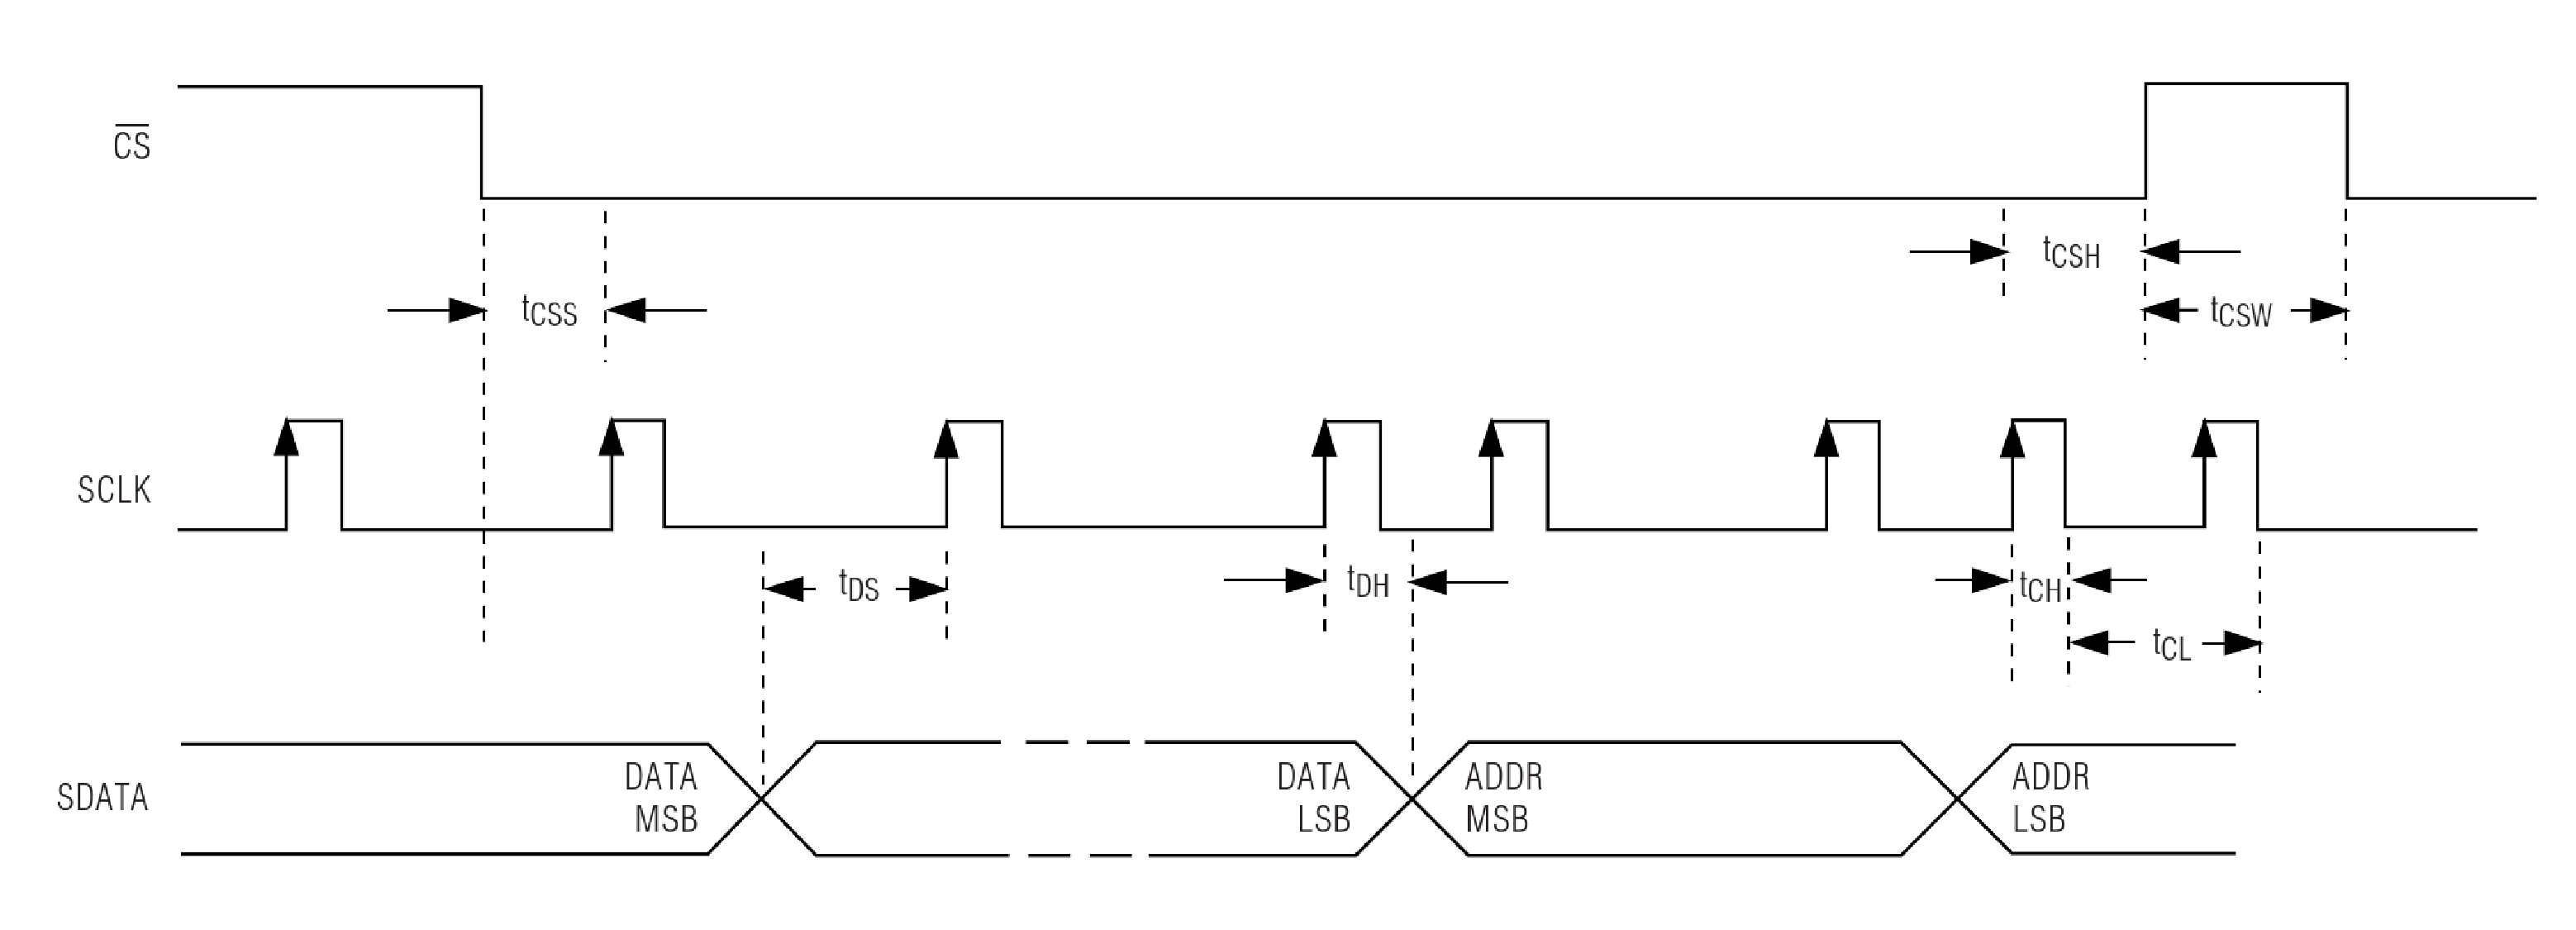
\includegraphics[width=1\linewidth]{./pics/gps_serial_times.eps}}
\caption{Временная диарамма serial-интерфейса GPS}
\end{figure}

\begin{table}[h]
\caption{Таблица 1. Временные требования для serial-интерфейса}
\label{tabular:serial-time}
\begin{tabular}{|c|p{250pt}|c|p{70pt}|}
 \hline  
  Символ & Параметр & Значение & Единица измерения  \\  
 \hline  
  $t_{css}$  & Время между падающим фронтом сигнала $\bar {CS}$ и передним фронтом сигнала SCLK	& 10 & нс  \\  
 \hline  
  $t_{ds}$   & Время установки данных на serial-линию	& 10 & нс \\  
 \hline  
  $t_{dh}$   & Время удержания данных на serial-линии	& 10 & нс \\  
 \hline  
  $t_{ch}$   & Время нахождения Сlock-сигнала serial-интерфейса в состоянии 1 & 25 & нс \\  
 \hline  
  $t_{cl}$   & Время нахождения Сlock-сигнала serial-интерфейса в состоянии 0 & 25 & нс \\  
 \hline  
  $t_{csh}$  & Время между крайним возрастающим фронтом сигнала SCLK и падающим фронтом сигнала $\bar {CS}$ & 10 & нс \\  
 \hline  
  $t_{csw}$  & Время $\bar {CS}$ в активном состоянии    & 1 & такт \\  
 \hline  
\end{tabular}
\end{table}

\begin{figure}[h]
\center{\includegraphics[width=1\linewidth]{./pics/gps_serial_clock_oscylloscope.eps}}
\caption{Clock-сигнал для serial-интерфейса GPS}
\end{figure}

\newpage
					% технологический раздел 
\section*{Введение}
Целью данного дипломного проекта является разработка и реализация программно-аппаратных средств
для захвата и сопровождения сигнала спутниковой навигации. Оборудования захвата радиосигналов является очень востребованным.
На данный момент оно применяется в научных разработках посвещенных анализу и улучшению алгоритмов определения координат 
приемника сигналов, а так же в таких специфических исследованиях, как определение погоды по уровню сигнала спутников.
При разработке данного программного-аппаратного комплекса возникают различные вредные психофизиологические факторы, влияющие
на программиста, которые рассматриваются в разделе “Безопасность жизнедеятельности”.  

\newpage

\setcounter{section}{3}
\section{Безопасность жизнедеятельности}

\subsection{Анализ пожарной опасности в помещении небольших размеров, где установлена вычислительная техника}

Пожары в ВЦ представляют особую опасность, так как сопряжены с большими материальными потерями.
Характерная особенность ВЦ - небольшие площади помещений. Как известно пожар может возникнуть при взаимодействии
горючих веществ, окисления и источников зажигания. В помещениях ВЦ присутствуют все три основные фактора,
необходимые для возникновения пожара. Горючими компонентами на ВЦ являются: строительные материалы для
акустической и эстетической отделки помещений, перегородки, двери, полы, перфокарты и перфоленты, изоляция кабелей и др.

Противопожарная защита - это комплекс организационных и технических мероприятий, направленных на обеспечение безопасности людей,
на предотвращение пожара, ограничение его распространения, а также на создание условий для успешного тушения пожара.

Источниками зажигания в ВЦ могут быть электронные схемы от ЭВМ, приборы, применяемые для технического обслуживания,
устройства электропитания, кондиционирования воздуха, где в результате различных нарушений образуются перегретые элементы,
электрические искры и дуги, способные вызвать загорания горючих материалов.

В современных ЭВМ очень высокая плотность размещения элементов электронных схем. В непосредственной близости
друг от друга располагаются соединительные провода, кабели. При протекании по ним электрического тока выделяется
значительное количество теплоты. При этом возможно оплавление изоляции. Для отвода избыточной теплоты от ЭВМ служа
системы вентиляции и кондиционирования воздуха. При постоянном действии эти системы представляют собой дополнительную
пожарную опасность. Энергоснабжение ВЦ осуществляется от трансформаторной станции и двигатель-генераторных агрегатов.
На трасформаторных подстанциях особую опасность представляют трансформаторы с масляным охлаждением. В связи с этим
предпочтение следует отдавать сухим транформатором. Пожарная опасность двигатель-генераторных агрегатов обусловленна
возможностью коротких замыканий, перегрузки, электрического искрения. Для безопасной работы необходим правильный
расчет и выбор аппаратов защиты. При поведении обслуживающих, ремонтных и профилактических работ используются
различные смазочные вещества, легковоспламеняющиеся жидкости, прокладываются временные электропроводники, ведут пайку
и чистку отдельных узлов. Возникает дополнительная пожарная опасность, требующая дополнительных мер пожарной защиты.
В частности, при работе с паяльником следует использовать несгораемую подставку с несложными приспособлениями
для уменьшения потребляемой мощности в нерабочем состоянии.

Для большинства помещений ВЦ установлена категория пожарной опасности В \cite{npb10503}. Одной из наиболее важных задач пожарной защиты
является защита строительных помещений от разрушений и обеспечение их достаточной прочности в условиях воздействия
высоких температур при пожаре. Учитывая высокую стоимость электронного оборудования ВЦ, а также категорию его
пожарной опасности, здания для ВЦ и части здания другого назначения, в которых предусмотрено размещение ЭВМ должны
быть 1 и 2 степени огнестойкости. Для изготовления строительных конструкций используются, как правило, кирпич,
железобетон, стекло, металл и другие негорючие материалы. Применение дерева должно быть ограниченно, а в
случае использования необходимо пропитывать его огнезащитными составами. В ВЦ противопожарные преграды в виде
перегородок из несгораемых материалов устанавливают между машинными залами.

\subsection{Оснащение помещения устойством для локального тушения пожаров}

К средствам тушения пожара, предназначенных для локализации небольших загораний, относятся пожарные стволы,
внутренние пожарные водопроводы, огнетушители, сухой песок, асбестовые одеяла и т. п. В зданиях ВЦ пожарные
краны устанавливаются в коридорах, на площадках лестничных клеток и входов. Вода используется для тушения пожаров
в помещениях программистов, библиотеках, вспомогательных и служебных помещениях. Применение воды в машинных залах
ЭВМ, хранилищах носителей информации, помещениях контрольно измерительных приборов ввиду опасности повреждения или
полного выхода из строя дорогостоящего оборудования возможно в исключительных случаях, когда пожар принимает
угрожающе крупные размеры. При этом количество воды должно быть минимальным, а устройства ЭВМ необходимо защитить
от попадания воды, накрывая их бризентом или полотном.

Для тушения пожаров на начальных стадиях широко применяются огнетушители. По виду используемого огнетушащего
вешества огнетушители подразделяются на следующие основные группы. Пенные огнетушители, применяются для тушения
горящих жидкостей, различных материалов, конструктивных элементов и оборудования, кроме электрооборудования,
находящегося под напряжением. Газовые огнетушители применяются для тушения жидких и твердых веществ, а также
электроустановок, находящихся под напряжением. В производственных помещениях ВЦ применяются главным образом
углекислотные огнетушители, достоинством которых является высокая эффективность тушения пожара, сохранность
электронного оборудования, диэлектрические свойства углекислого газа, что позволяет использовать эти огнетушители
даже в том случае, когда не удается обесточить электроустановку сразу. Для обнаружения начальной стадии
загорания и оповещения службу пожарной охраны используют системы автоматической пожарной сигнализации (АПС).
Кроме того, они могут самостоятельно приводить в действие установки пожаротушения, когда пожар еще не достиг
больших размеров. Системы АПС состоят из пожарных извещателей, линий связи и приемных пультов (станций).
Эффективность применения систем АПС определяется правильным выбором типа извещателей и мест их установки.
При выборе пожарных извещателей необходимо учитывать конкретные условия их эксплуатации: особенности помещения и
воздушной среды, наличие пожарных материалов, характер возможного горения, специфику технологического процесса и т.п.

Особое внимание уделяется пожарной безопасности, так как пожары в ВЦ сопряжены с опасностью для человеческой
жизни и большими материальными потерями.

В соответствии с "Типовыми правилами пожарной безопасности для промышленных предприятий" залы ЭВМ, помещения
для внешних запоминающих устройств, подготовки данных, сервисной аппаратуры, архивов, копировально множительного
оборудования и т.п. необходимо оборудовать дымовыми пожарными извещателями. В этих помещениях в начале пожара
при горении различных пластмассовых, изоляционных материалов и бумажных изделий выделяется значительное количество
дыма и мало теплоты. В других помещениях ВЦ, в том числе в машинных залах дизель генераторов и лифтов, трансформаторных
и кабельных каналах, воздуховодах допускается применение тепловых пожарных извещателей. Объекты ВЦ кроме АПС необходимо
оборудовать установками стационарного автоматического пожаротушения. Наиболее целесообразно применять в ВЦ установки
газового тушения пожара, действие которых основано на быстром заполнении помещения огнетушащим газовым веществом с
резким смижением содержания в воздухе кислорода.

Меры по пожарной профилактики:
\begin{itemize}
\item строительно-планировочные;
\item технические;
\item способы и средства тушения пожаров;
\item организационные.
\end{itemize}

Строительно-планировочные определяются огнестойкостью зданий и сооружений (выбор материалов конструкций: сгораемые, несгораемые,
трудносгораемые) и предел огнестойкости — это количество времени, в течение которого под воздействием огня не нарушается
несущая способность строительных конструкций вплоть до появления первой трещины.

Все строительные конструкции по пределу огнестойкости подразделяются на 8 степеней от 1/7 ч до 2ч.

Для помещений ВЦ используются материалы с пределом стойкости от 1-5 степеней. В зависимости от степени огнестойкости определены
наибольшие дополнительные расстояния от выходов для эвакуации при пожарах (5 степень — 50 м).

Технические меры:
\begin{itemize}
\item это соблюдение противопожарных норм при эвакуации систем вентиляции, отопления, освещения, эл. обеспечения и т.д.
\item использование разнообразных защитных систем;
\item соблюдение параметров технологических процессов и режимов работы оборудования.
\end{itemize}

Организационные меры — проведение обучения по пожарной безопасности, соблюдение мер по пожарной безопасности.

Средства пожаротушения:
\begin{description}
\item[a)]Ручные
	\begin{itemize}
	\item огнетушитель порошковый;
	\item огнетушитель углекислотный, бромэтиловый
	\end{itemize}

\item[б)] Cистема пожаротушения ручного действия (кнопочный извещатель).
Для ВЦ используются тепловые датчики-извещатели типа ДТЛ, дымовые радиоизотопные типа РИД.
\end{description}

Для ВЦ используются огнетушители углекислотные ОУ, ОА (создают струю распыленного бром этила).

Способ соединения датчиков в системе эл. пожарной сигнализации с приемной станцией может быть — параллельным (лучевым);
— последовательным (шлейфным).

Норма оснащения помещения категории В  переносными огнетушителями составляет(предельная защищаемая площадь 200м$^2$) 
\cite{bjd421}:
\begin{description}

	\item[a)] порошковые огнетушители:
		\begin{itemize}
		\item 2 огнетушителя весом 2кг для категории пожаров A, B, C, D, E;
		\item 1 огнетушитель весом 8кг для категории пожаров A, B, C, D, E;
		\end{itemize}
	\item[б)] 	углекислотные огнетушители:
		\begin{itemize}
		\item 2 огнетушителя весом 3кг для категории пожаров E;
		\end{itemize}

\end{description}

\subsection{Экологическая оценка проектируемой компьютерной техники}
Внедрение в промышленность новых, более эффективных промышленных процессов, резкое повышение продуктивности и расширение
масштабов производства потребовали увеличения затрат материальных и энергетических ресурсов, что, в свою очередь,
привело к росту отрицательного воздействия на окружающую среду. Основными проблемами по решению задач защиты окружающей
среды являются: совершенствование технологических процессов и разработка нового оборудования с меньшим уровнем выброса
примесей и отходов в окружающую среду, также необходимо уменьшить влияние таких факторов как шум при работе, излучение
высокочастотных электромагнитных полей, сильный разогрев и т.п.

Более 80\% общей трудоемкости производства вычислительной техники связано с производством печатных плат.
При изготовлении печатных плат происходит загрязнение воздушного пространства парами свинца \cite{bjd43}, а соединения кислот и
щелочей загрязняют сточные воды предприятия. При производстве плат должны предусматриваться эффективные средства
защиты окружающей среды от возможного загрязнения.

Лидер в области бессвинцового производства – японская промышленность. Начало его организации было положено в декабре 1997 года
после издания закона о контроле утилизации веществ, содержащих свинец. Их подлежало герметично упаковывать перед захоронением
для предотвращения выщелачивания свинца на поверхность.

В апреле 1998 года Япония начала реализацию проекта по изучению бессвинцового процесса, названного NEDO, целью которого было
создание базы данных по бессвинцовым припоям для удобства выбора материала и разработки технологии пайки.
Общий бюджет проекта составил 350 млн. иен за два года. Участники проекта – представители крупнейших японских
производителей электронных систем, компонентов и сплавов. В результате уже к 2001 году следующие крупнейшие японские
производители сумели сформировать собственные планы полного отказа от свинцовой пайки:
\begin{itemize}
\item Matsushita (Panasonic) еще в октябре 1998 года выпустила первый компактный мини-дисковый плеер, выполненный с
	использованием только бессвинцового сплава Sn/Ag/Bi/Cu. К 2001 году компания провозгласила полный отказ от применения свинца;
\item Sony в 2001 году полностью исключила применение свинца при монтаже устройств с повышенной плотностью;
\item Toshiba к 2000 году прекратила использовать свинец при производстве мобильных телефонов;
\item Hitachi к 1999 году сократила использование свинца на 50\% по сравнению с 1997-м. К 2001-му вся продукция компании
	выпускалась уже без применения свинца.
\end{itemize}

Гальванические работы сопряжены с использованием больших объёмов воды для приготовления растворов электролитов и
промывочных операций. Поэтому сточные воды в этих случаях значительно загрязнены ядовитыми химическими веществами.
Кроме того, воздух, удаляемый от технологического гальванического оборудования, содержит большое количество вредных
веществ в различных агрегатных состояниях: капель жидком, паро- и газообразном.Технологические процессы сварки и
пайки сопровождаются выделением пыли и токсичных газов, а сточные воды могут загрязняться механическими примесями,
кислотами. Процесс получения функционально завершённого изделия заканчивается сборочными операциями. Отрицательное
воздействие на окружающую среду процессов сборки менее ощутимо. Однако и в этих случаях при проведении
санитарно-гигиенической обработки производственных помещений в сточные воды могут попадать различные нежелательные примеси.

В настоящее время широко используются пассивные методы защиты, суть которых сводится к ограничению количества
загрязняющих окружающую среду выбросов, т.е. улавливанию пылегазовыделений, выбрасываемых в атмосферу, очистка
сточных вод от примесей и т.п. При производстве модулей должны использоваться пассивные фильтры, которые основаны
на способности пористых материалов задерживать частицы примесей при движении дисперсных сред. Частицы примесей оседают
на входной части фильтроэлемента, помещённого в корпус. Осаждение частиц происходит в результате совокупного действия
эффекта касания, диффузионных, инерционных гравитационных процессов. Для очистки воздуха от туманов кислот, щелочей,
масел и других жидкостей используются волоконные фильтры, принцип действия которых основан на осаждении капель на
поверхности материалов и последующего отекания жидкостей под воздействием сил тяжести.

При загрязнении сточных вод маслосодержащим и примесями, помимо отстаивания и фильтрования, применяется также
процесс флотации. Очистка вод флотацией заключается в интенсификации процесса маслопродуктов при их частиц
пузырьками воздуха, попадающего в сточную воду. Таким образом, наиболее перспективной формой защиты окружающей
среды от вредного воздействия является «безотходная» технология и комплекс природоохранных мероприятий в
технологических процессах от обработки сырья до использования готовой продукции.

\newpage

\section*{Заключение}
В разделе "Безопасность жизнедеятельности" был проведен анализ пожарной опасности в помещении небольших размеров,
где установлена ВТ. Разработаны мероприятия по оснащению помещения устройством для локального тушения пожаров. Дана
экологическая оценка проектируемой компьютерной техники.

\newpage
					% архиважно биля 
%\section{ОРГАНИЗАЦИОННО-ЭКОНОМИЧЕСКИЙ РАЗДЕЛ}
\subsection{Планирование разработки программных средств с построением графика}
Целью дипломного проекта является разработка программного комплекса (ПК) оценки трудоемкости объектно-ориентированных программ.
В данном разделе определяется трудоёмкость и затраты на создание ПК, а так же производится расчёт основных технико-экономических
показателей проекта.

\subsubsection*{Определение трудоемкости и продолжительности работ по созданию ПК}
Процесс разработки включает: обзор и анализ программных средств схожей тематики, анализ и выбор программных продуктов для
создания программы; отладка; испытание. В свою очередь каждый из этих этапов можно подразделить на отдельные под этапы.
Согласно ГОСТ 23501.1-79 регламентируются следующие стадии проведения исследования:

\begin{itemize}
	\item техническое задание – ТЗ (ГОСТ 23501.2-79);
	\item эскизный проект – ЭП (ГОСТ 23501.5-80);
	\item технический проект – ТП (ГОСТ 23501.6-80);
	\item рабочий проект – РП (ГОСТ 23501.11-81);
	\item внедрение – ВП (ГОСТ 23501.15-81).
\end{itemize}

Планирование стадий и содержания работ осуществляется в соответствии с \cite{bibl51}. На всех стадиях проведения исследования
выполняются следующие виды работ, перечень которых показан в таблице ~\ref{tab:eco1}.

% http://users.sdsc.edu/~ssmallen/latex/longtable.html
\begin{center}
\begin{longtable}{|l|l|}
\caption{Состав работ и стадии разработки ПК} \label{tab:eco1} \\ \hline
\multicolumn{1}{|c|}{\textbf{Стадии разработки}}    &   \multicolumn{1}{c|}{\textbf{Перечень работ}} \\ \hline
\multicolumn{1}{|c|}{\textbf{1}}    &   \multicolumn{1}{|c|}{\textbf{2}} \\ \hline
\endfirsthead

%\multicolumn{2}{c} %
%{{\bfseries \tablename \thetable{} -- continued from previous page}} \\
\multicolumn{2}{|l|}{{Продолжение таблицы ~\ref{tab:eco1}}} \\ %\hline
\hline \multicolumn{1}{|c|}{\textbf{1}} &
%\multicolumn{1}{c|}{\textbf{Triple chosen}} &
\multicolumn{1}{c|}{\textbf{2}} \\ \hline 
\endhead

%\multicolumn{2}{|r|}{{}} \\ %\hline
%\hline \multicolumn{2}{|r|}{{Continued on next page}} \\ %\hline
\endfoot

\hline
\endlastfoot
		Техническое задание & \begin{parbox}{5in} {
						\begin{itemize}
							\item постановка задачи;
							\item подбор литературы;
							\item сбор исходных данных;
							\item определение требований к системе;
							\item определение стадий, этапов и сроков разработки ПК;
						\end{itemize} }  
					\end{parbox} \\
	\hline
		Эскизный проект & \begin{parbox}{5in} {
					\begin{itemize} 
						\item анализ программных средств схожей тематики;
						\item разработка общей структуры ПК;
						\item разработка структуры программы по подсистемам;
						\item документирование;
					\end{itemize} }
				\end{parbox} \\
	\hline
		Технический проект & \begin{parbox}{5in} {
					\begin{itemize} 
						\item определение требований к ПК;
						\item выбор инструментальных средств;
						\item определение свойств и требований к аппаратному обеспечению;
					\end{itemize} } 
				\end{parbox} \\
	\hline
		Рабочий проект & \begin{parbox}{5in} {
					\begin{itemize} 
						\item программирование;
						\item тестирование и отладка ПК;
						\item разработка программной документации;
						\item согласование и утверждение программы и методики испытаний;
					\end{itemize} }
				\end{parbox} \\
	\hline
		Внедрение & \begin{parbox}{5in} {
					\begin{itemize}
						\item ;
						\item ;
						\item ;
						\item ;
					\end{itemize} }
				\end{parbox} \\
\end{longtable}
\end{center}

Трудоемкость выполнения работ по созданию ПК  на каждой из стадий определяется в соответствии с \cite{bibl52, bibl53}.

Трудоемкость разработки ПК определяется по сумме трудоемкости этапов и видов работ, оцениваемых экспертным путем в
человеко-днях, и носит вероятностный характер, так как зависит от множества трудно учитываемых факторов.

Трудоемкость каждого вида работ определяется в соответствии с методическими указаниями \cite{bibl53} по формуле:

\begin{equation}
t_i = \frac{3\cdot{t_{min}} + 2\cdot{t_{max}}}{5},
\label{eq:eco1}
\end{equation}
где:	$t_{min}$ - минимально возможная трудоемкость выполнения отдельного вида работ в человеко-днях; \\
	$t_{max}$ - максимально возможная трудоемкость выполнения отдельного вида работ в человеко-днях.

Продолжительность каждого вида работ в календарных днях ${(T_i)}$ определяется по формуле \cite{bibl53}:

\begin{equation}
T_i = \frac{t_i}{\mbox{Ч}_i}\cdot{K_{\mbox{вых}}},
\label{eq:eco2}
\end{equation}
где:	${t_i}$ - трудоемкость работы, человек-дней; \\
	${\mbox{Ч}_i}$ - численность исполнителей, человек; \\
	${K_{\mbox{вых}}}$ - коэффициент, учитывающий выходные и праздничные дни: \\

\begin{equation}
T_i = \frac{K_{\mbox{кап}}}{K_{\mbox{раб}}},
\label{eq:eco3}
\end{equation}
где:	${K_{\mbox{кап}}}$ - число календарных дней;
	${K_{\mbox{раб}}}$ - рабочие дни.

Для расчёта принимается среднее значение ${K_{\mbox{вых}} = 1.45}$. 

Полный список видов и этапов работ по созданию ПС, экспертные оценки и расчетные величины их трудоемкости,
а также продолжительность каждого вида работ, рассчитанные по формулам (\ref{eq:eco1}) и (\ref{eq:eco2}) представлены
в таблице ~\ref{tab:eco2}.

% table

%\begin{center}
%\begin{longtable}{|l|l|}
%\caption{Расчёт трудоёмкости и продолжительности работ по созданию ПС} \label{tab:eco2} \\ \hline

%\multicolumn{1}{|p{1cm}|}{\textbf{ 1 }} &
%\multicolumn{1}{|p{5cm}|}{\textbf{2}} &
%\multicolumn{1}{|p{5cm}|}{\textbf{3}} \\ \hline
%& \multicolumn{1}{|p{1cm}|}{\textbf{Количество исполнителей, чел.}} \\ \hline
%\multicolumn{1}{|c|}{\textbf{Продолжительность, календарные дни}} \\ \hline

%\multicolumn{1}{|c|}{\textbf{1}}    &   \multicolumn{1}{c|}{\textbf{2}} \\ \hline

%\endfirsthead

%\multicolumn{2}{|l|}{{Продолжение таблицы ~\ref{tab:eco1}}} \\ %\hline
%\hline \multicolumn{1}{|c|}{\textbf{1}} &
%\multicolumn{1}{c|}{\textbf{2}} \\ \hline 
%\endhead
%\endfoot

%\hline
%\endlastfoot

% ================================================================

%\end{longtable}
%\end{center}

% end of the table

Таким образом, общая трудоёмкость разработки ПС составляет  88 человеко-дней, а их продолжительность – 112 календарных дней.

\subsubsection*{Построение ленточного графика разработки ПС}
В качестве инструмента планирования работ используем ленточный график. Ленточный график является удобным, простым и наглядным
инструментом для планирования работ. Он представляет собой таблицу, где перечислены  работы и длительность выполнения каждой
из них. Продолжением таблицы является линейный график, построенный в масштабе, наглядно показывающий продолжительность
каждой работы в виде отрезков прямых,  располагающихся в соответствии с последовательностью выполнения работ.

Ленточный график разработки ПС, построенный на основе данных табл. ~\ref{tab:eco2} приведён на рисунке ~\ref{pic:line_graphic} 
Он позволяет наглядно представить логическую последовательность и взаимосвязь отдельных работ, сроки начала и окончания работ,
соблюдение которых обеспечит своевременное выполнение проекта и разработку программных средств.

% Picture here

\subsection{Расчет сметы затрат на  разработку ПС}
Сметная стоимость проектирования и внедрения программы включает в себя  затраты, определяемые по формуле (\ref{eq:eco_smeta}):

\begin{equation}
C_{\mbox{пр}} = C_{\mbox{осн}} + C_{\mbox{доп}} + C_{\mbox{соц}} + C_{\mbox{м}} + C_{\mbox{маш.вр.}} + C_{\mbox{н}},
\label{eq:eco_smeta}
\end{equation}
где:	${C_{\mbox{пр}}}$ - стоимость разработки ПС; \\
	${C_{\mbox{м}}}$ - затраты на используемые материалы; \\
	${C_{\mbox{осн}}}$ - основная заработная плата исполнителей; \\
	${C_{\mbox{доп}}}$ - дополнительная заработная плата исполнителей, учитывающая потери времени на отпуска и болезни
		(принимается в среднем 10\% от основной заработной платы); \\
	${C_{\mbox{соц}}}$ - единый социальный налог (ЕСН), представляющий собой отчисления во внебюджетные фонды
		государственного социального страхования (пенсионный фонд, фонд обязательного медицинского страхования,
		фонд социального страхования). Рассчитывается в соответствии с установленной ставкой ЕСН как 26\% от
		основной и дополнительной заработной платы; \\
	${C_{\mbox{н}}}$ - накладные расходы включают затраты на управление, уборку, ремонт, электроэнергию, отопление и
		другие хозяйственные расходы (принимаются в размере 60\% от основной и дополнительной заработной платы);
	${C_{\mbox{маш.вр.}}}$ - стоимость машинного времени. \\

\subsubsection*{Основная заработная плата исполнителей}
На статью «Заработная плата» относят заработную плату научных, инженерно-технических и других работников,
непосредственно участвующих в разработке ПС. Расчёт ведётся по формуле (\ref{eq:eco_zarplata}):
\begin{equation}
\mbox{З}_{\mbox{исп}} = \mbox{З}_{\mbox{ср}} \cdot{T},
\label{eq:eco_zarplata}
\end{equation}
где:	${\mbox{З}_{\mbox{исп}}}$ - заработная плата исполнителей (руб.); \\
	${\mbox{З}_{\mbox{ср}}}$ -  средняя дневная тарифная ставка работника организации разработчика ПС (руб./чел.дни); \\
	${T}$ - трудоёмкость разработки ПС (чел.дни). \\

${\mbox{З}_{\mbox{ср}}}$ определяется по формуле (\ref{eq:eco_zsr}):
\begin{equation}
\mbox{З}_{\mbox{ср}} = \frac{C}{\mbox{Ф}_{\mbox{мес}}},
\label{eq:eco_zsr}
\end{equation}
где:	${C}$ - месячная зарплата работника (руб./мес.); \\
	${\mbox{Ф}_{\mbox{мес}}}$ - среднее количество рабочих дней в месяце (20дн.). \\

Расчёт затрат на основную заработную плату разработчиков ПС приведен в таблице \ref{tab:eco_zarplata}.

\begin{center}
\begin{longtable}{|c|c|c|c|c|c|}
\caption{Затраты на заработную плату} \label{tab:eco_zarplata} \\ \hline
\multicolumn{1}{|c|}{\textbf{№}} & \multicolumn{1}{c|}{\textbf{Исполнитель}} & 
\multicolumn{1}{p{2.5cm}|}{\textbf{Оклад, руб./мес.}} &   \multicolumn{1}{p{2.5cm}|}{\textbf{Оклад, руб./день}} & 
\multicolumn{1}{p{3.5cm}|}{\textbf{Трудоемкость, чел. дней}} & \multicolumn{1}{p{2cm}|}{\textbf{Сумма, руб.}} \\ \hline

\multicolumn{1}{|c|}{\textbf{1}} &   \multicolumn{1}{c|}{\textbf{2}} & 
\multicolumn{1}{c|}{\textbf{3}} &   \multicolumn{1}{c|}{\textbf{4}} & 
\multicolumn{1}{c|}{\textbf{5}} & \multicolumn{1}{c|}{\textbf{6}} \\ \hline
\endfirsthead

\multicolumn{6}{|l|}{{Продолжение таблицы ~\ref{tab:eco_zarplata}}} \\ %\hline
\hline
\multicolumn{1}{|c|}{\textbf{1}} &   \multicolumn{1}{c|}{\textbf{2}} & 
\multicolumn{1}{c|}{\textbf{3}} &   \multicolumn{1}{c|}{\textbf{4}} & 
\multicolumn{1}{c|}{\textbf{5}} & \multicolumn{1}{c|}{\textbf{6}} \\ \hline
\endhead

\endfoot

\hline
\endlastfoot

1. & Руководитель & 35000 & 1750 & 10 & 17500 \\ \hline
2. & Инженер & 21000 & 1050 & 78 & 81900\\ \hline
 & Итого ${C_{\mbox{осн}}}$ & - & - & 88 & 99400 \\

\hline

\end{longtable}
\end{center}

\subsubsection*{Дополнительная заработная плата}
Дополнительная заработная плата на период разработки ПС рассчитывается относительно основной и составляет 10\% от её величины:

\begin{equation}
C_{\mbox{доп}} = C_{\mbox{осн}} \cdot 0.1,
%\label{eq:eco_smeta}
\end{equation}

\subsubsection*{Расчёт отчислений на социальное страхование}
Отчисления на социальное страхование рассчитываются относительно выплаченной заработной платы (суммы основной и
дополнительной заработной платы). Составляют 26\%:

\begin{equation}
C_{\mbox{соц}} = (C_{\mbox{доп}} + C_{\mbox{осн}}) \cdot 0.26,
%\label{eq:eco_smeta}
\end{equation}

\subsubsection*{Расчёт расходов на материалы}
На эту статью относят все затраты на магнитные носители данных, бумагу, для печатных устройств, канцтовары и др.
Затраты по ним определяются по экспертным оценкам. Расчёт расходов на материалы приведён в табл. \ref{tab:eco_zatnm}

\begin{center}
\begin{longtable}{|c|c|c|c|}
\caption{Затраты на заработную плату} \label{tab:eco_zatnm} \\ \hline
\multicolumn{1}{|c|}{\textbf{№}} & \multicolumn{1}{c|}{\textbf{Материалы}} & 
\multicolumn{1}{c|}{\textbf{Кол-во, шт}} &   \multicolumn{1}{c|}{\textbf{Стоимость, руб.}} \\ \hline

\multicolumn{1}{|c|}{\textbf{1}} &   \multicolumn{1}{c|}{\textbf{2}} & 
\multicolumn{1}{c|}{\textbf{3}} &   \multicolumn{1}{c|}{\textbf{4}} \\ \hline
\endfirsthead

\multicolumn{4}{|l|}{{Продолжение таблицы ~\ref{tab:eco_zatnm}}} \\ %\hline
\hline
\multicolumn{1}{|c|}{\textbf{1}} &   \multicolumn{1}{c|}{\textbf{2}} & 
\multicolumn{1}{c|}{\textbf{3}} &   \multicolumn{1}{c|}{\textbf{4}} \\ \hline
\endhead

\endfoot

\hline
\endlastfoot

1. & Блокноты & 2 &   \\ \hline
2. & Другие канцтовары & - &  \\ \hline
 & Итого ${C_{\mbox{м}}}$ & & XXX \\

\hline

\end{longtable}
\end{center}

\subsubsection*{Накладные расходы}
На статью «Накладные расходы» относят расходы, связанные с управлением и организацией работ, содержанием помещений
(освещение, отопление, уборка и т.д.). Накладные расходы рассчитываются относительно основной заработной платы. Величина
накладных расходов принимается равной 60\% от основной зарплаты исполнителей. Формула расчёта (\ref{eq:eco_naklr})

\begin{equation}
C_{\mbox{н}} = C_{\mbox{осн}} \cdot K,
\label{eq:eco_naklr}
\end{equation}
где:	${C_{\mbox{н}}}$ - накладные расходы (руб.); \\
	${C_{\mbox{осн}}}$ - основная заработная плата исполнителей (руб.);
	${K}$ - коэффициент учёта накладных расходов (К=0,6).

${C_{\mbox{н}} = XXX \cdot 0.6 = YYY}$

\subsubsection*{Расчёт стоимости машинного времени}
Включает затраты на машинное время, необходимое для разработки ПС, расходы на подготовку и приобретение материалов
научно-технической информации, расходы на использование средств связи. Расчет затрат на машинное время осуществляется
по формуле (\ref{eq:eco_pricePC}):

\begin{equation}
C_{\mbox{маш.вр.}} = K_{\mbox{маш.вр.}} \cdot 3_{\mbox{маш.вр.}},
\label{eq:eco_pricePC}
\end{equation}
где:	${K_{\mbox{маш.вр.}}}$ - средняя стоимость одного часа машинного времени (берется 50руб./час); \\
	${3_{\mbox{маш.вр.}}}$ - машинное время, используемое на проведение исследования.	

Необходимое количество машинного времени для реализации проекта по разработке программы рассчитывается по формуле (\ref{eq:eco_zmashvr}):

\begin{equation}
3_{\mbox{маш.вр.}} = t_i \cdot T_{\mbox{см}} \cdot T_{\mbox{ср.маш.}},
\label{eq:eco_zmashvr}
\end{equation}
где:	${t_i}$ - трудоёмкость работ, человек-дней;
	${T_{\mbox{см}}}$ - продолжительность рабочей смены (при пятидневной рабочей неделе - 8 часов);
	${T_{\mbox{ср.маш.}}}$ - средний коэффициент использования оборудования (берется 0.7).

Тогда: ${3_{\mbox{маш.вр.}} = FIXME}$ (маш.час)

Стоимость машинного времени составит: ${C_{\mbox{маш.вр.}} = FIXME}$ (руб.)

Результаты расчета затрат на проектирование программных средств представлены в таблице \ref{tab:eco_smeta}.

\begin{center}
\begin{longtable}{|c|c|c|c|c|}
\caption{Затраты на заработную плату} \label{tab:eco_smeta} \\ \hline
\multicolumn{1}{|c|}{\textbf{№}} & \multicolumn{1}{c|}{\textbf{Наименование статей}} & 
\multicolumn{1}{c|}{\textbf{Обозначение}} &   \multicolumn{1}{c|}{\textbf{Сумма, руб}} & 
\multicolumn{1}{c|}{\textbf{В \% к итогу}} \\ \hline

\multicolumn{1}{|c|}{\textbf{1}} &   \multicolumn{1}{c|}{\textbf{2}} & 
\multicolumn{1}{c|}{\textbf{3}} &   \multicolumn{1}{c|}{\textbf{4}} & 
\multicolumn{1}{c|}{\textbf{5}} \\ \hline
\endfirsthead

\multicolumn{5}{|l|}{{Продолжение таблицы ~\ref{tab:eco_smeta}}} \\ %\hline
\hline
\multicolumn{1}{|c|}{\textbf{1}} &   \multicolumn{1}{c|}{\textbf{2}} & 
\multicolumn{1}{c|}{\textbf{3}} &   \multicolumn{1}{c|}{\textbf{4}} & 
\multicolumn{1}{c|}{\textbf{5}} \\ \hline
\endhead

\endfoot

\hline
\endlastfoot

1. & Основная заработная плата & ${C_{\mbox{осн.}}}$ & 99400 & 45 \\ \hline
2. & Доп. заработная плата & ${C_{\mbox{доп.}}}$ & 9940 & 4 \\ \hline
3. & Отчисления на соц. нужды & ${C_{\mbox{соц.}}}$ & 28428 & 13 \\ \hline
4. & Материалы & ${C_{\mbox{мат.}}}$ & 2550 & 13 \\ \hline
5. & Стоимость маш. времени & ${C_{\mbox{маш.вр.}}}$ & 2550 & 13 \\ \hline
6. & Накладные расходы & ${C_{\mbox{н}}}$ & 2550 & 13 \\ \hline
   & Итого: & ${C_{\mbox{пр}}}$ & 2550 & 13 \\ 

\hline

\end{longtable}
\end{center}

Таким образом, себестоимость разработки ПС составляет FIXME руб.

Данная программа может быть реализована на рынке. При расчётном количестве реализованных программ – n, оптовая цена программы
(${\mbox{Ц}_{\mbox{опт}}}$) может быть рассчитана по формуле:

\begin{equation}
\mbox{Ц}_{\mbox{опт}} = \frac{\mbox{С}_{\mbox{пр}}}{n} + \mbox{П}_i,
%\label{eq:eco_zarplata}
\end{equation}
где:	${\mbox{С}_{\mbox{пр}}}$ - себестоимость разработки программы; \\
	${\mbox{П}}$ - прибыль, определяется по формуле:

\begin{equation}
\mbox{П}_i = Y_p \cdot \frac{C_{npi}}{n} \cdot 100,
%\label{eq:eco_zarplata}
\end{equation}
где:	${Y_p}$ -  средний уровень рентабельности (принимается Yр= 20\%);\\

Таким образом, при среднем расчётном количестве реализованных программ n = 10 оптовая цена ПС составит: \\
${\mbox{Ц}_{\mbox{опт}} = FIXME}$ руб. \\

Отпускная оптовая цена реализации программы потребителям должна включать налог на добавленную
стоимость (НДС) и рассчитывается по формуле:

\begin{equation}
\mbox{Ц}_{\mbox{отп}} = \mbox{Ц}_{\mbox{опт}} + \mbox{НДС},
%\label{eq:eco_zarplata}
\end{equation}
где НДС – налог на добавленную стоимость,  рассчитывается в соответствии с действующей ставкой этого
налога - 18\% от оптовой цены программы:

\begin{center}
${\mbox{НДС} = FIXME \mbox{(руб.)}}$ \\
${\mbox{Ц}_{\mbox{отп}} = FIXME \mbox{(руб.)}}$
\end{center}

Таким образом, отпускная цена программы составит  31407  руб.,  в том числе НДС – 4791 (руб.).

\subsection{Расчет основных технико-экономических показателей использования программного продукта}
В настоящей дипломной работе  разработаны алгоритмы и проведена программная реализация эксперимента по
автоматизации защиты локальной вычислительной сети. Использование этих алгоритмов и программных средств 
позволит повысить эффективность защиты локальной вычислительной сети, соответственно повысится эффективность
работы администратора, следящего за бесперебойной работой сети, что способствует более качественному уровню
обслуживания пользователей.



\newpage
				% экономический раздел 
%\section{ДРУГИЕ РАЗДЕЛЫ ПРОЕКТА}

%==========================================================================================

\subsection{Руководство пользователя по работе с приложением}

Для запуска в фоне используется сторонняя программа screen. Порядок работы с программой screen:

\begin{enumerate}
\renewcommand{\labelenumi}{\arabic{enumi}.}
\item запуск программы screen из терминала.
\item запуск board daemon, путем запуска скрипта \textbf{./start}.
\item отсоединение от screen-терминала с помощью команды \textbf{Ctrl+a+d}.
\end{enumerate}
О успешном старте board daemon свидетельствует надпись \textbf{[rs232\_process] Process...}

Если пользователю нужно создать дамп по запросу, ему необходимо выполнить следующую цепочку операций:
\begin{enumerate}
\renewcommand{\labelenumi}{\arabic{enumi}.}
\item c помощью команды \textbf{ps -waux | grep board\_daemon} узнать pid процесса board daemon
\item выполнить команду \textbf{kill -USR1 pid}, где pid - номер процесса, полученный на предыдущем шаге 
\end{enumerate}


%==========================================================================================

\subsection{Руководство программиста}
Клонирование исходных текстов проекта осуществляется с помощью системы контроля версий GIT.  Для клонирования
необходимо иметь доступ в интернет и установленный GIT. Клонирование осуществляется командой \textbf{gitclone http://github.com/venik/gps\_project.git}.
После этого на компьютере программиста появится папка gps\_project в которой будет находится последняя версия исходных кодов программного продукта.
В дереве исходного кода существуют папки doc, src, mngmt. 

Папка src содержит все исходные коды проекта. В ней содержатся папки hardware и software. В папке software находятся все программные модули проекта:
сервер платы, парсер конфигурационных файлов, исходные коды ФАПЧ для Matlab. В папке hardware находятся исходные коды модулей для ПЛИС микросхемы Xilinx:
исходный код арбитра платы, контроллера SRAM-памяти, модуля тестирования SRAM-памяти, модуля сохранения полученного сигнала, модуля программирования GPS
микросхемы, контроллер RS-232 интерфейса, модуль парсера двоичного протокола. \\
hardware/arbiter.vhd - арбитр платы выполняет основную управляющую функцию. \\
hardware/rs-232/rs232\_rx\_new.vhd, hardware/rs-232/rs232\_tx\_new.vhd - реализация RS-232 интерфейса. \\
hardware/sram\_M5M5V208FP-85L/sram.vhd - реализация контроллера SRAM-памяти. \\
hardware/mem\_test/test\_sram.vhd - модуль тестирования SRAM-памяти. \\
hardware/gps/gps\_main.vhd, hardware/gps/gps\_serial.vhd - модуль программирования режимов GPS микросхемы, реализация последовательного 
	интерфейса программирования GPS-микросхемы. \\
hardware/top\_level/top\_level.vhd - реализация мультиплексной шины адреса и данных SRAM-микросхемы. \\
src/hardware/board - файлы разводки платы. \\
software/board\_daemon - реализация сервера платы. \\
software/include - заголовочные файлы парсера конфигурационных файлов, заголовочные файлы протоколов. \\
software/manage\_scripts - исходные коды публикации дампов в публичные источники.
software/gpstool - исходные коды для среды Matlab используемые в обработке данных GNSS. \\
software/rs232\_client - исходные коды отладочного клиента платы. \\


В папке mngmt находятся скрипты управления деревом исходного кода проекта.

В папке doc находится документация на плату и документация на сервисное ПО.

%==========================================================================================

\subsection{Руководство системного программиста}
Для использования данных программных средств на компьютере должна быть установлена операционная система Gentoo Linux для сервера платы и MS Windows XP с 
математическим пакетом Matlab для модуля сопровождения сигнала. 
Для установки и работы с программными средствами обозначим минимальные требования к конфигурации компьютера: процессор с тактовой частотой 1 ГГц, память 1024 Мб,
жёсткий диск объёмом 10 Гб, объём видеопамяти 32 Мб. 

Board daemon требует прав root или suid бита для исполнения(требуется для открытия RS-232 порта). Запуск демона осуществляется из консоли командой
\begin{center}
\textbf{./board\_daemon -c default\_cfg}
\end{center}
где через -c ключ указывается конфигурационный файл. В конфигурационном файле указывается режим работы GPS-микросхемы, скрипт публикации дампа и имя RS-232 порта.
Пример конфигурационного файла представлен ниже:

\hrulefill \\
    \# GPS Registers \\
    addr0=a2939a3 \\
    addr1=855028c \\
    addr2=0x6aff1dc \\
    addr3=0x9ec0008 \\
    addr4=0x0c00080 \\
    addr5=0x8000070 \\
    addr6=0x8000000 \\ 
    addr7=0x10061b2 \\
    addr8=0x1e0f401 \\
    addr9=0x14c0402 \\
\\
    \# GUI-server thread \\
    gui\_tcpport=1234 \\
\\
    \# Board-server thread \\
    rs232\_portname=/dev/ttyUSB0 \\
    upload\_script=../manage\_scripts/store\_flush.sh

\hrulefill

Через addrX задается значение для программирование регистра X (X = 0..9). Так же задается порт для подключения графического конфигуратора,
имя RS-232 порта и имя скрипта публикации дампа.

\newpage
					% хзн раздел 
%\addcontentsline{toc}{chapter}{Литература}
\begin{thebibliography}{99}
% 1.1
%\bibitem{yacenkov} Яценков В.С. Основы спутниковой навигации. Системы GPS NAVSTAR и ГЛОНАСС.-М:Горячая линия-Телеком, 2005.-272 с.:ил.
%\bibitem{tsui} Bao-Yen Tsui, J., Fundamentals of Global Positioning System Receivers: A Software Approach, 2nd ed. (New York: John Wiley \& Sons, Inc., 2004).
%\bibitem{gpsyellow} Grewal, M. S., Weill, L. R., and Andrews, A. P., Global Positioning Systems, Inertial Navigation, and Integration, John Wiley \& Sons, New York, NY, 2001.
%\bibitem{gps} Borre, Kai, Akos, Dennis, Bertelsen, Nicolaj, Rinder, Peter \& Holdt Jensen, Soren (2007) A Software-Defined GPS and Galileo Receiver. Single-Frequency Approach. Birkhauser Boston, 200 pages

%1.2
%\bibitem{ni_acq} http://www.ni.com/dataacquisition/whatis.htm.
%\bibitem{ni_article} http://zone.ni.com/devzone/cda/tut/p/id/7189
%\bibitem{seamax_overview} http://www.seasolve.com/mobile-wimax-signal-analyzer.html
%\bibitem{seamax_pdf} http://www.seasolve.com/pdf/wimax-brochure.pdf
%\bibitem{soft_gps} http://kom.aau.dk/project/softgps/
%\bibitem{soft_gps1} http://www.nsl.eu.com/primo\_order.php

% special
\bibitem{sram} M5M5V208FP,VP,RV,KV,KR data sheet
\bibitem{gps_max} MAX2769 data sheet


% section 4 - BJD
% 4.1
%\bibitem{sec41}ГОСТ 27331
% 4.2
%\bibitem{sec42} Журнал-каталог "ПОЖАРНАЯ АВТОМАТИКА 2004"
%\bibitem{bjd1} ГОСТ 12.3.046
%\bibitem{bjd2} ГОСТ 15150
%\bibitem{bjd3} ПУЭ-98

% 4.3

\end{thebibliography}
					% 
\end{document}
